\section{Experimenting with Word2Vec Embeddings}

In this section you will be experimenting with pre-trained Word2Vec embeddings in a Google CoLab python notebook. We highly recommend opening the notebook in a Google Chrome browser. To get started, you will need to access the notebook here: \url{https://bit.ly/3xhJq2B}.

\textbf{Google CoLab notebooks are shared and saved just like Google Docs}. Upon visiting the notebook, go to``File $>$ Save a copy in Drive''. You will then be able to see a copy of the notebook in a folder named “Colab Notebooks” inside your Google Drive. This is the file you should work with.

\begin{itemize}
    \item The notebook is divided into individual cells. When running code in the notebook, one can run one cell at a time, and the output of the code will populate under the cell. The values of any variables used in this cell will be stored and can be used when running future cells. The variable values will be written over if the cell is run again.  
    
    \item One of the cells loads in the Word2Vec embeddings. This takes a good bit of time (10-15 mins)! We highly recommend that you run this cell once and then use the stored word vectors in your future experiments without reloading the embeddings. The notebook is set up in a fashion conducive to this use.
\end{itemize}
\clearpage

% ONLY UNCOMMENT WHEN GRADESCOPE ONLINE ASSESSMENT FEATURE IS DOWN
% This remainder of this homework is a series of multiple choice and True/False questions related to the CoLab notebook exercise described on the previous page.

% {\bf How to submit:}  Even though these are not coding questions, you will submit your response to
% each question in the |src-quiz/submission.py| file.  This file will act as
% your 'bubble sheet' for multiple choice questions in this course.  A sample response
% might look like this:

% \begin{center}
% 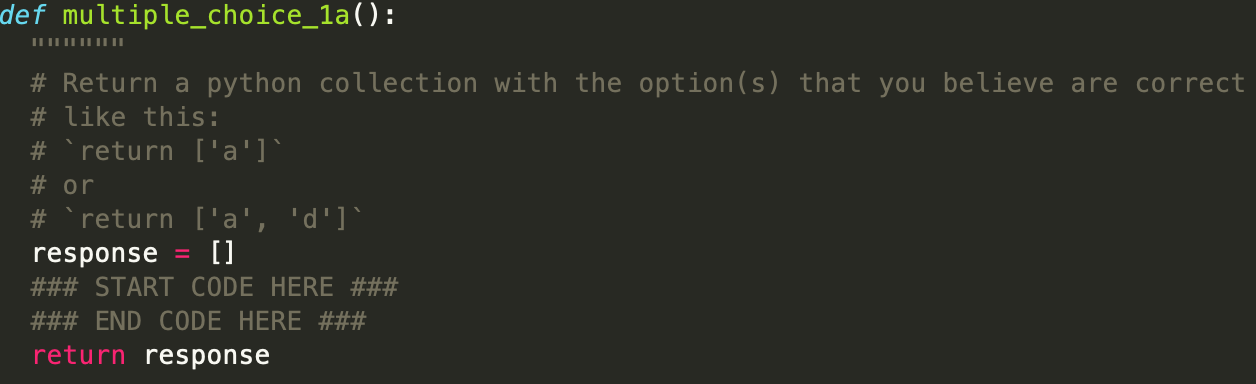
\includegraphics[width=1\textwidth]{sample_question_empty.png}
% \end{center}

% If you believe that |a| and |b| are the correct responses to this question, you
% will type |response = [`a', `b']| between the indicated lines like this:

% \begin{center}
% 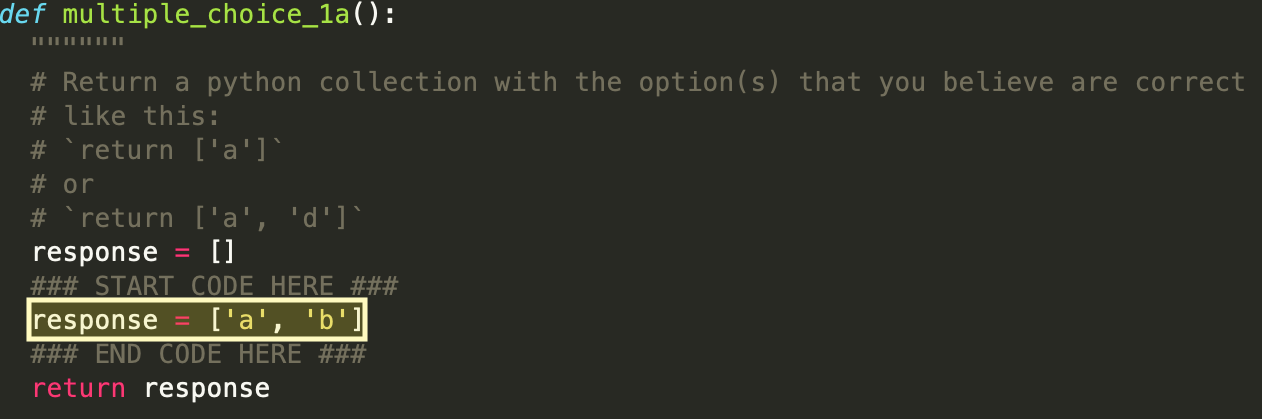
\includegraphics[width=1\textwidth]{sample_question_complete.png}
% \end{center}

% {\bf How to verify your submission:}
% You can run the student version of the autograder locally like all coding
% problem sets.  In the case of this problem set, the helper tests will verify
% that your responses are within the set of possible choices for each question
% (e.g. the helper functions will flag if you forget to answer a question of if
% you respond with |[`a', `d']| when the choices are |[`a', `b', `c']|.)  See the
% front pages of this assignment for instructions to run the autograder.
% \clearpage

Once you have opened the Google CoLab notebook, begin following the steps there and inputting your answers into the Gradescope Online Assessment |A1 (Google Colab) Online Assessment|.
For more instructions on how to submit to the GradeScope Online Assesment, please review this video tutorial: \url{https://bit.ly/3BbYu4g}.

\begin{enumerate}[1.]
\item \points{1quiz}

Please input answer to question 1 of the Gradescope online assessment |A1 (Google Colab) Online Assessment|.

We provide a similar plot to the one you generated in part one of the assignment, this time using Word2Vec embeddings.

\begin{center}
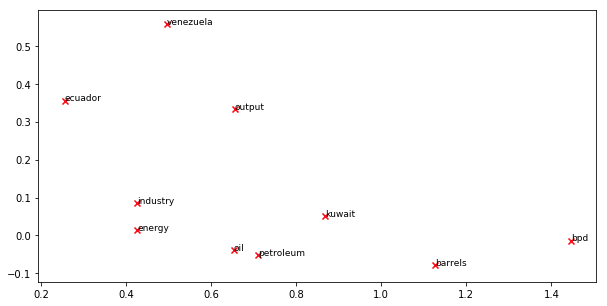
\includegraphics[width=1\textwidth]{embeddings_plot.png}
\end{center}

Why aren't countries ``venezuela'',``ecuador'' and ``kuwait'' clustered together in the Word2Vec plot while as they in your co-occurence plot? - Select all the reasonable possibilities

\begin{enumerate}[a.]
\item Word2Vec was trained on a larger dataset in which the countries did not always appear in the same contexts as the small dataset used to compute the co-occurence matrix.
\item Word2Vec recognizes that the words are countries, and thus groups them by geography, while the co-occurence method does not. 
\item For the Word2Vec embeddings, the first two principal components may represent attributes of the words "venezuela", "ecuador" and "kuwait" which are not similar, while in the co-occurence embeddings, they may represent attributes of the words which are similar. 
\item In the Word2Vec corpus, the countries "venezuela", "ecuador" and "kuwait" do not appear in each others’ contexts, so they are not similar in the embeddings.
\end{enumerate}

% ### START CODE HERE ###
% ### END CODE HERE ###

\item \points{2quiz}

Please input answers to question 2.1 - 2.8 of the Gradescope online assessment |A1 (Google Colab) Online Assessment|.

For the following homonyms, respond True if the top 10 most similar words represent more than one meaning for the homonym and False otherwise. These are case sensitive so please make sure to input the word exactly as specified below:

\begin{enumerate}[a.]
\item left
\item nuts
\item pen
\item right
\item drive
\item rose
\item mean
\item saw
\end{enumerate}

% ### START CODE HERE ###
% ### END CODE HERE ###

\item \points{3quiz}

Please input answer to question 3 of the Gradescope online assessment |A1 (Google Colab) Online Assessment|.

Why do you think many of the homonyms you tried did not represent more than one meaning? - Select all the reasonable possibilities.

\begin{enumerate}[a.]
\item A different word vector is trained for each meaning of the homonym, so synonyms for a particular meaning of the word will be most similar depending on the which vector we are using for the original word.

\item In some scenarios, one meaning of the homonym is much more common in the training data than the other meanings, resulting in the vector for the homonym is much closer to words from one meaning than the other(s).

\item When a particular meaning of a homonym is much more common than the others, the algorithm that trains the word vectors is able to recognize this and only learns to encode one of the definitions in the word vector.
\end{enumerate}

% ### START CODE HERE ###
% ### END CODE HERE ###

\item \points{4quiz}

Please input answer to question 4.1 - 4.8 of the Gradescope online assessment |A1 (Google Colab) Online Assessment|.

Mark True if the antonyms pair has a smaller cosine distance than the synonyms pair. Mark False otherwise. Please make sure to input the words exactly as specified below: 
\begin{enumerate}[a.]
\item \textsf{happy, sad $\vert$ happy, cheerful}
\item \textsf{right, wrong $\vert$ right, correct}
\item \textsf{big, small $\vert$ big, large}
\item \textsf{good, bad $\vert$ good, nice}
\item \textsf{day, night $\vert$ day, daytime}
\item \textsf{insane, sane $\vert$ insane, crazy}
\item \textsf{several, one $\vert$ several, numerous}
\item \textsf{antonym, synonym $\vert$ antonym, opposite}
\end{enumerate}

% ### START CODE HERE ###
% ### END CODE HERE ###

\item \points{5quiz}

Please input answer to question 5 of the Gradescope online assessment |A1 (Google Colab) Online Assessment|.

Why do you think there are times where synonym-antonym pairs have a smaller cosine distance than the synonym-synonym pairs? - Select all the reasonable possibilities.

\begin{enumerate}[a.]
\item Sometimes, the synonym-antonym pair has two words that are found with much higher frequency in the corpus than the other synonym word. The word vectors capture this frequency, making the synonym-antonym pair more similar than the synonym-synonym pair.

\item In some cases, the antonym is a homonym and carries multiple meanings, some of which may have definitions slightly similar to the synonym, making them overall fairly similar.

\item We may find that the synonym-antonym words are actually used in similar contexts, more so than the synonym-synonym words, making the synonym-antonym words more similar.
\end{enumerate}

% ### START CODE HERE ###
% ### END CODE HERE ###

\item \points{6quiz}

Please input answer to question 6.1 - 6.12 of the Gradescope online assessment |A1 (Google Colab) Online Assessment|.

Mark True if the word vectors are able to successfully complete the analogy. Mark False otherwise. These are case sensitive so please make sure to input the word exactly as specified below:

\begin{enumerate}[a.]
\item \textsf{man:king::woman:QUEEN}
\item \textsf{air:plane::sea:BOAT}
\item \textsf{happy:laugh::sad:CRY} %FUNNY
\item \textsf{cat:kitten::dog:PUPPY}
\item \textsf{France:Paris::Germany:BERLIN}
\item \textsf{carnivore:meat::herbivore:VEGETABLES} %MEATS
\item \textsf{dog:bark::cat:MEOW} %MEOW
\item \textsf{bat:baseball::racquet:TENNIS}
\item \textsf{mosque:Islam::church:CHRISTIANITY}
\item \textsf{long:longer::short:SHORTER}
\item \textsf{longer:longest::more:MOST}
\item \textsf{talk:talked::help:HELPED}
\end{enumerate}

% ### START CODE HERE ###
% ### END CODE HERE ###

\item \points{7quiz}

Please input answer to question 7 of the Gradescope online assessment |A1 (Google Colab) Online Assessment|.

What factors might contribute to the biases observed in the word vectors presented in the notebook examples? - Select all the reasonable possibilities.

\begin{enumerate}[a.]
\item Text data is generated by people, and thus word vectors trained on a corpus are prone to have the same biases of the people who generated the corpus 
\item The training corpus may have many instances of sentences that relate certain races, genders, etc. to certain properties or behaviours
\end{enumerate}

% ### START CODE HERE ###
% ### END CODE HERE ###

\end{enumerate}
